\documentclass[10pt,a4paper]{article}
\usepackage[latin1]{inputenc}
\usepackage{amsmath}
\usepackage{amsfonts}
\usepackage{amssymb}
\usepackage{graphicx}
\usepackage{float}

\usepackage{caption}
\usepackage{subcaption}

\begin{document}
\section{February 29th 2016}
\begin{itemize}
\item Show the area with a colorbar showing height
\item Fix problem with z-values close to infinity or below zero
\item Look at the spill point analysis for 
\end{itemize}

\subsection{Overview of the landscape that we have data over}
\begin{figure*}[h!]
    \centering
    \begin{subfigure}[h]{0.65\textwidth}
        \centering
        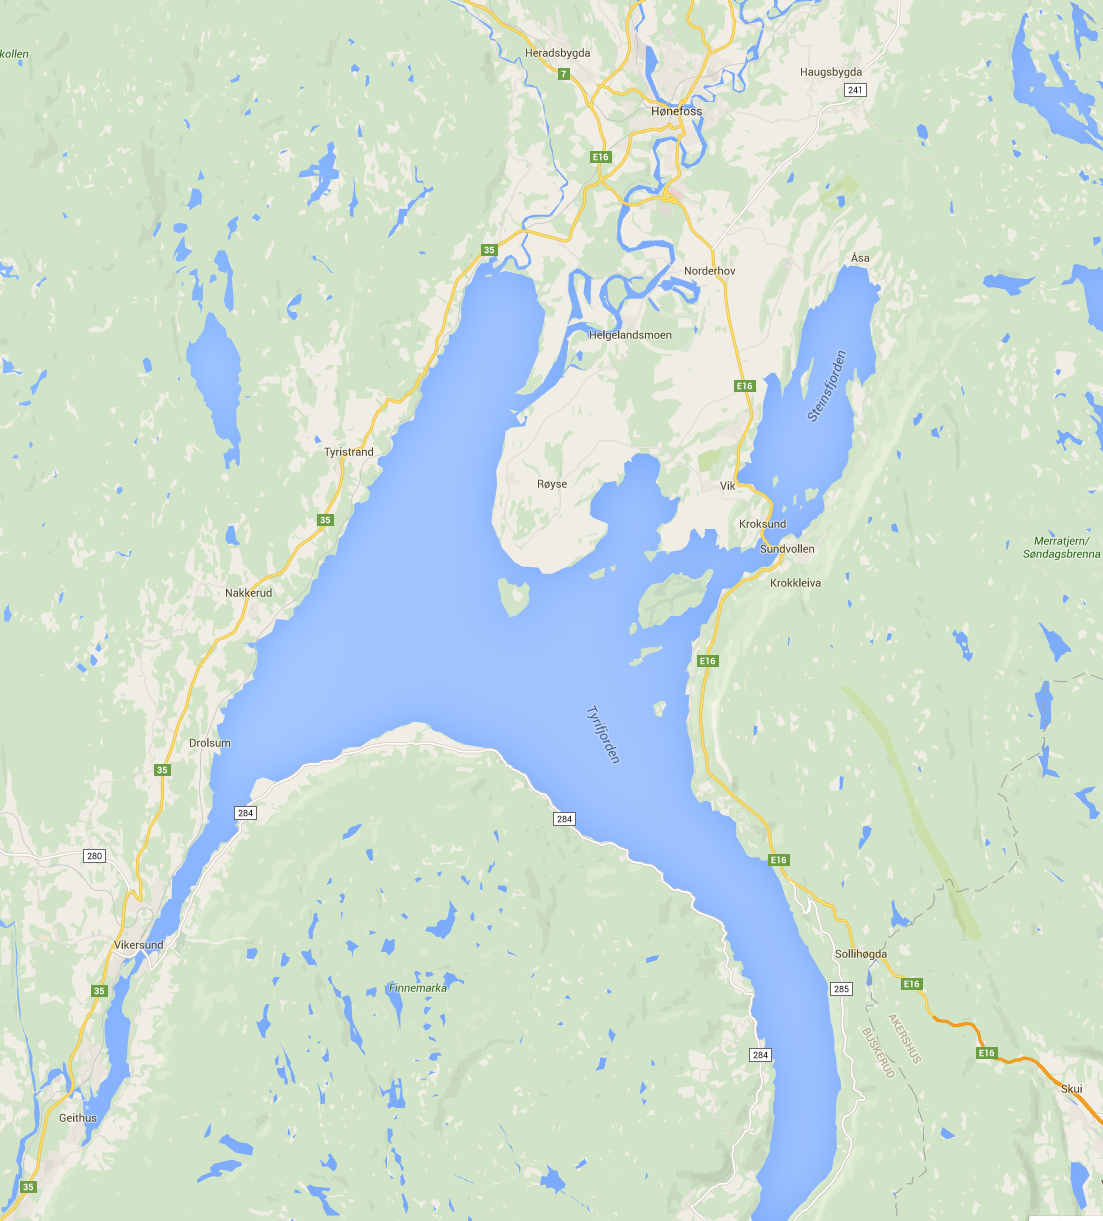
\includegraphics[height=1\textwidth]{map_area.png}
        \caption{The landscape as seen in Google Maps.}
    \end{subfigure}%
    ~ 
    \begin{subfigure}[h]{0.65\textwidth}
        \centering
        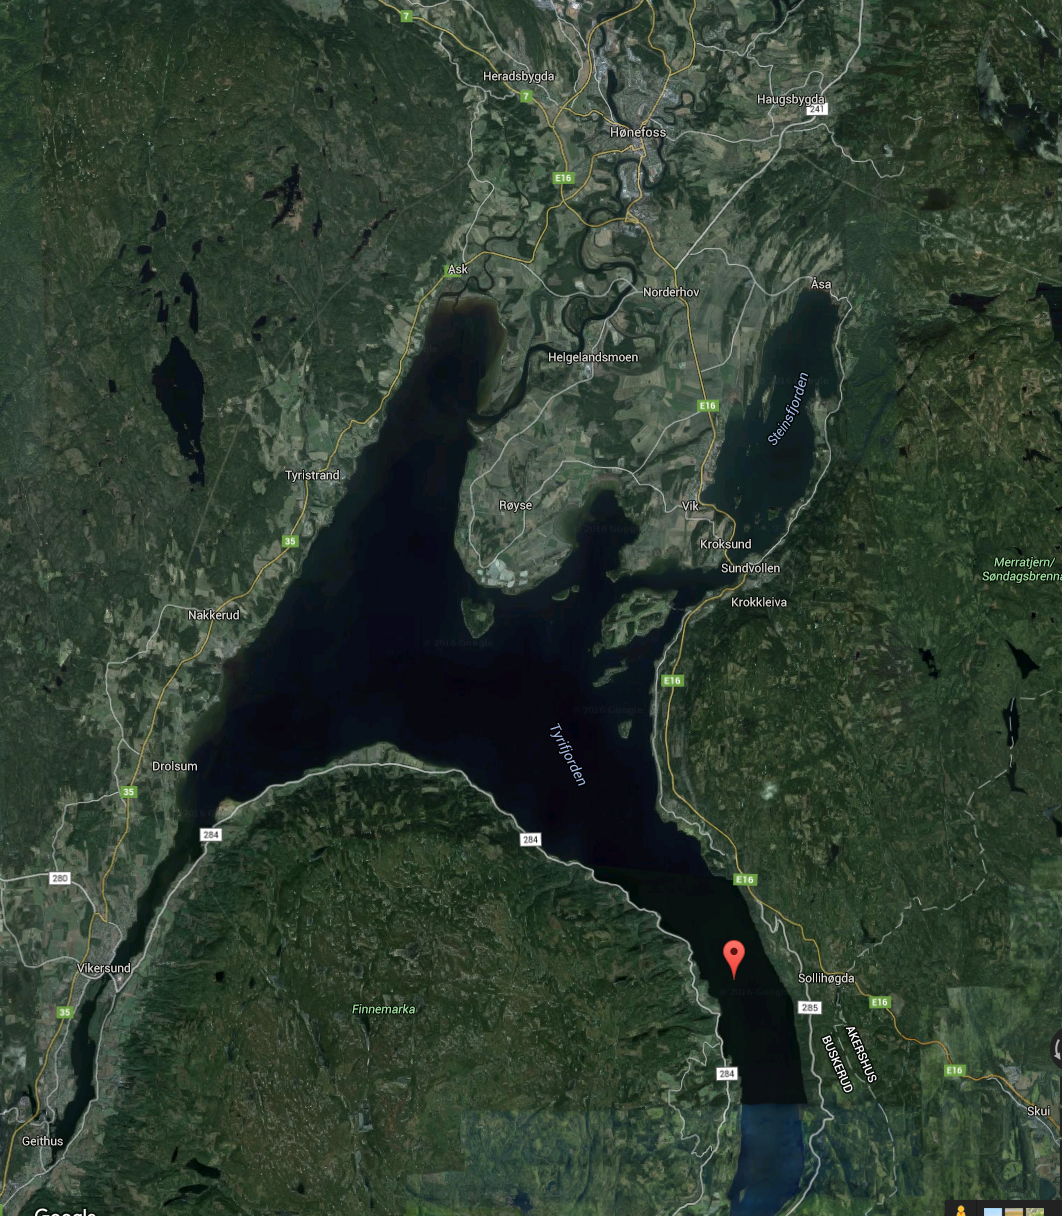
\includegraphics[height=1\textwidth]{earth_map.png}
        \caption{The landscape as seen in Google Earth.}
    \end{subfigure}
    \caption{Two different views of the landscape.}
\end{figure*}




\begin{figure}[H]
  \centering
    \includegraphics[width=1.1\textwidth]{landscape_hoh.eps}
  \caption{The landscape with height shown. Black is 0 meters above sea level. White is 1200 masl.}
\end{figure}

\subsection{Problem: z-values close to infinity or below zero}
For a given area we have a matrix $z$ which gives the height for some coordinate in the area. In some cases there might be $z$-values which for some reason are clearly wrong, e.g. the value is larger than the tallest point in Norway. In those cases we need to remove them. One way of doing this is the one below.
\begin{align}
zvals(zvals > 2469) = \textrm{NaN}\\
zvals(zvals < 0) = \textrm{NaN}\\
zvals = inpaint\_nans(double(zvals))
\end{align}
All $z$-values larger than a threshold will be set to NaN and given as input to a function that finds NaN-elements in a matrix and interpolates them with neighboring points. The function can be found in the link below:\\
 http://www.mathworks.com/matlabcentral/fileexchange/4551-inpaint-nans


\end{document}